\section{Prototypes vs actual implementation}
In \autoref{sec:prototypes-design} we introduced some of our prototypes.
In this section we will compare some of these designs with the final implementation.

\begin{figure}[H]
    \begin{subfigure}{0.5\textwidth}
    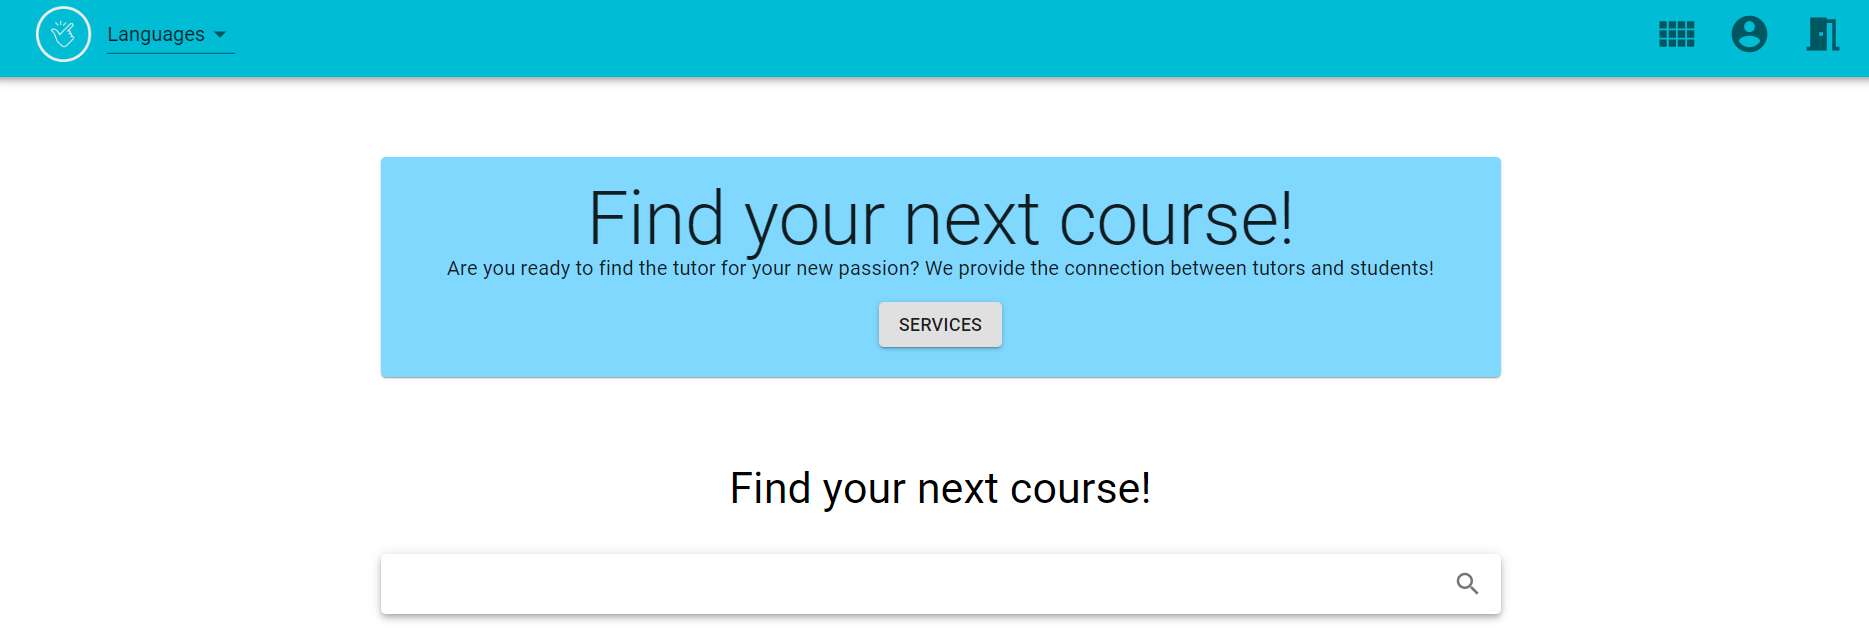
\includegraphics[width=1\linewidth, height=5cm]{prototypes/landingpageupper.png} 
    \caption{The upper part of the implemented landing page}
    \label{fig:landing-page-upper}
    \end{subfigure}
    \begin{subfigure}{0.5\textwidth}
        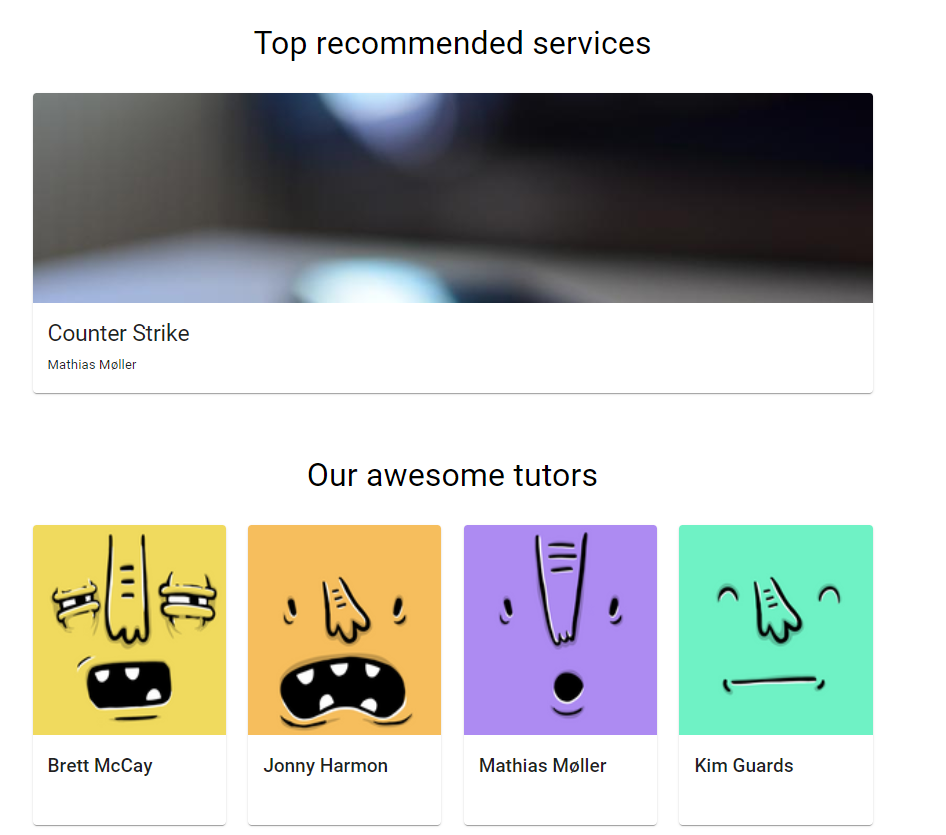
\includegraphics[width=1\linewidth, height=5cm]{prototypes/landingpagelower.png}
    \caption{The lower part of the impemented landing page}
    \label{fig:landing-page-lower}
    \end{subfigure} 
    \caption{This figure shows how the implemented landing page looks}
    \label{fig:landing-page-implemented}
\end{figure}
\noindent
In \autoref{fig:landing-page} we showed how the prototype for the landing page looked.
The implemented version of the landing page, shown in \autoref{fig:landing-page-implemented}. , ended looking a bit different.
The layout of the prototype and the implemented version is somewhat the same. 
The same functionality is there, where some of the tutors are shown and the user is able to search for a course. 
A new addition in the implemented version is the recommended services that show a couple of services that the current user might be interested in. 
If the user is not logged in, the top rated services are shown instead. 
The implemented landing page is a bit less bloated with information as well and the design is simpler.

\begin{figure}[H]
    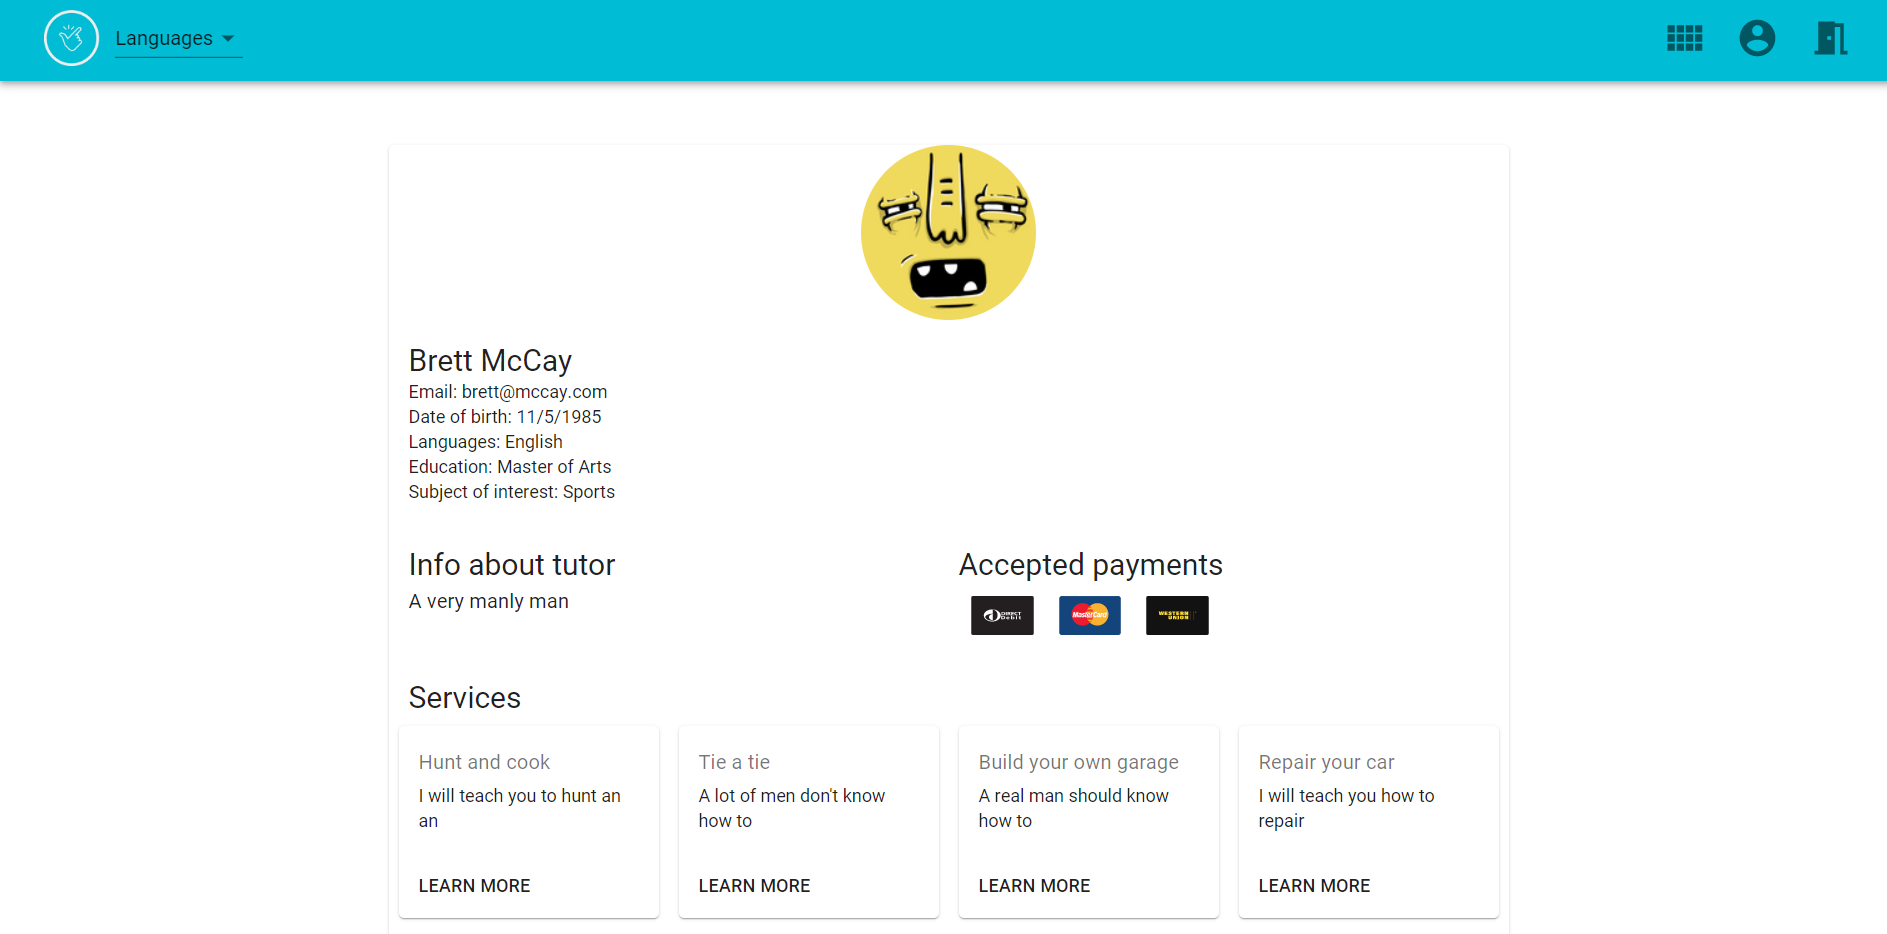
\includegraphics[width=1\linewidth, height=5cm]{prototypes/tutorinfoimplemented.PNG} 
    \caption{The implemented view of the tutor information page}
    \label{fig:tutor-info-implemented}
\end{figure}
\noindent
In \autoref{fig:view-information-on-tutor} we showed the prototype for viewing the information on a tutor.
Because of time limitation and changes in priority during the project, some of the features available on the prototype were not implemented. The page shows all the basic information about a tutor and it also shows the services that the tutor provides.
Since tutor materials and the calendar was not implemented, it did not make sence to render available material and appointments on the tutor's page.